% Chapter 2

\chapter{LITERATURE REVIEW OF GEOMETRIC MODELING} % Main chapter title

\label{Literature Review} % Change X to a consecutive number; for referencing this chapter elsewhere, use \ref{ChapterX}

\lhead{Chapter 2. \emph{Literature Review}} % Change X to a consecutive number; this is for the header on each page - perhaps a shortened title

%----------------------------------------------------------------------------------------
%      INTRODUCTORY PARAGRAPHS
%----------------------------------------------------------------------------------------
\hspace{30} With the advent of computers which could perform millions of floating
point operations in unit time and which are still growing faster, researchers who
believed computers could aid the processes of mechanical design and
manufacturing were faced with a critical issue – how to represent physical
reality using computer software. They sought the best data structures to
represent this reality and the most appropriate algorithms to manipulate these representations.

\hspace{30} BRL-­CAD supports a wide variety of geometric representations including an 
extensive set of traditional implicit primitive shapes as well as explicit primitives
made from collections of uniform B­spline surfaces, non­uniform rational B­spline (NURBS)
surfaces, n­on-manifold   geometry   (NMG)   and purely faceted polygonal mesh geometry.
Consequently, in this chapter, we review the existing work done by scholars in the 
field of geometric modeling which have been applied to the development of BRL-­CAD. 
First of all, it introduces the issue of representation and the notion of representation
 schemes.Then, it summarizes developments in wireframe modeling, surface modeling, solid
modeling and non­-manifold modeling (aka non­manifold geometry or nmg for short) with a keen
 eye on the algorithms underlying them.

\hspace{30} As we progress in our literature review from older forms of geometric
modeling to newer ones, we will discover that representation schemes were
closely linked to algorithmic efficiency and that it has always been normal to
expect designers to switch to newer ones in response to the improvements in
algorithmic performance.Despite these enhancements in algorithmic efficiency
within the designer community, we cannot say with complete certainty whether
traditional representation schemes can be relegated to the background. We
can only conclude that old and new representation paradigms co­exist and that
research led to representation schemes which supplemented the repertoire of
geometric modeling.  

%-----------------------------------------------------------------------------------------

%----------------------------------------------------------------------------------------
%	SECTION 1
%----------------------------------------------------------------------------------------

\section{Representation Schemes}

A representation $\textbf{\mathfrak{R}}$ of a solid or representation for short is a subset of
three­-dimensional Euclidean space denoted $\mathbb{E}^3$ which models a physical solid.  
According to [5], Requicha and Tilove stated that point set topology provided a
formal language for describing the geometric properties of solids and they also  
threw more light on the mathematical characteristics of solids such as a solid's
interior, boundary, complement, closure, boundedness and regularity.
Requicha [4] insisted that to be computationally useful, a representation should  
formally capture the following properties ;

\begin{itemize}
\item \textit{\textbf{Rigidity:}} Representations should have an invariant configuration
irrespective of their location and orientation.
\item \textit{\textbf{Homogeneity:}} A representation should have an interior.
\item \textit{\textbf{Finiteness:}} A representation must occupy a finite amount of space.
\item \textit{\textbf{Boundary   determinism:}} A representation must unambiguously determine
the interior of that solid.
\item \textit{\textbf{Closure}}: Representations of solids which are manipulated by rigid
motions and regularized boolean operations should produce representations of solids too.
\end{itemize}
These formal characteristics leave representations no choice than to be
bounded, closed, regularized and semi­analytic, hence their coinage r­sets
according to [5]. An \textit{\textbf{r-­set}} is simply a regular and bounded set in $\mathbb{E}^3$.

\hspace{30} A representation scheme is simply a relation between physical solids and their representations which can be characterized by the following properties;
\begin{itemize}
\item \textit{\textbf{Domain}}: A representation scheme must represent quite a number of useful geometric solids. 
\item \textit{\textbf{Unambiguity}}: A representation scheme should produce representations which intuitively capture the properties of the physical solid so that it can be easily distinguished from other representations.
\item \textit{\textbf{Uniqueness}}: A representation scheme should uniquely represent a solid object within a software's database.  
\item \textit{\textbf{Validity}}: Representation schemes should yield representations of solids which do not exist or are valid.  
\item \textit{\textbf{Closure}}: A Representation scheme which transforms (reflects, scales, rotates) a representation should yield other representations too.
\item \textit{\textbf{Compactness}}: Representation schemes should yield representations which save space and allow efficient algorithms to   determine desirable physical characteristics.
\end{itemize}
%--------------------------------------------------------------------------------------------------
%	WIREFRAME MODELING
%-----------------------------------------------------------------------------------------------------
\section{Wireframe Modeling}

For rectilinear objects whose edges are straight lines and whose faces are planar, the ordered pair of vertices
 $\textbf{\mathfrak{V}} \in \mathbb{E}^3$ and edges $\textbf{\mathfrak{E}} \in \mathbb{E}^3$ denoted by $(\textbf{\mathfrak{V}} , \textbf{\mathfrak{E}})$ is the object's wireframe.  
In a practical sense, it is the skeleton of an object wherein joints are vertices
and bones are edges. In [6], a six ­step algorithm to generate an object's
wireframe was developed wherein an object's wireframe was represented by a vertex table and an edge table. 
Although the work in [6] had drawbacks such as not checking the validity of input data, wireframe modeling has always provided designers with a chance to experiment with the final result of their models through sketching and it is frequently used to preview complex models. However, the use of only edge information left wireframe models ambiguous
on rectilinear polyhedra talk less of topological ones. Figure 2.1 below shows the wireframe of a sphere in greyscale.

%--------------------------------------------------------------------------------------------

\begin{figure}[htbp]
\centering
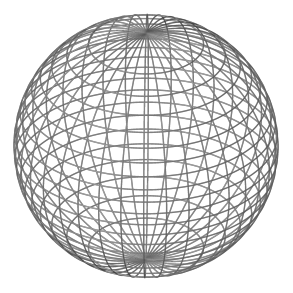
\includegraphics[trim=0.1cm 0.3cm 0.5cm 0.5cm, clip=true, totalheight=0.5\textheight]{Figures/Sphere.png}
\caption[A wireframe of a sphere]{A wireframe of a sphere}
\label{Sphere}
\end{figure}

%--------------------------------------------------------------------------------------------

%----------------------------------------------------------------------------------------
%	SURFACE MODELING
%----------------------------------------------------------------------------------------

\section{Surface Modeling}

After breakthroughs in wireframe modeling, research efforts in geometric modeling were directed 
towards extending the geometric coverage of CAD packages by incorporating complex free­form surfaces
 and curves. In this section, we emphasize on algebraic surfaces and curves used within BRL­-CAD 
as it is the basis for Bezier surfaces and NURBS.

%--------------------------------------------------------------------------------------------

\begin{figure}[htbp]
\centering
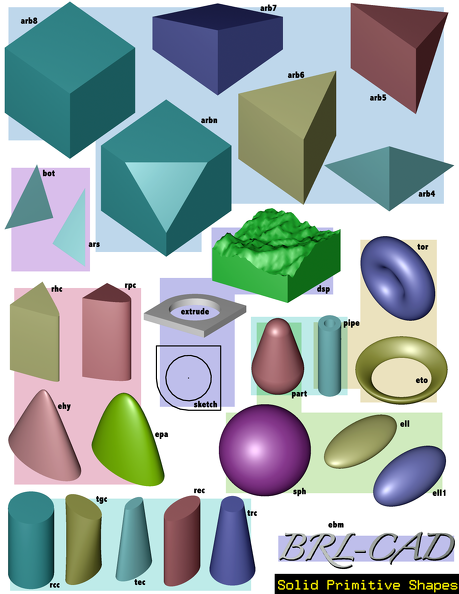
\includegraphics[trim=0.1cm 0.3cm 0.5cm 0.5cm, clip=true, totalheight=0.5\textheight]{Figures/Primitives.png}
\caption[BRL­CAD Solid Primitive Shapes]{BRL­CAD Solid Primitive Shapes}
\label{Primitives}
\end{figure}

%--------------------------------------------------------------------------------------------

Figure 2.2 above shows a collection of some primitives used within the BRL-­CAD package before the heart-­shaped primitive   was developed – several of which are implicitly and/or parameterically represented by algebraic equations.On the BRL-­CAD's   ideas page[7], there is a list of primitives which have not yet been implemented such as the Steiner surface, the ring 
cyclide surface, the quartoid, Wallis' conical edge solid, etc.  

%----------------------------------------------------------------------------------------------------
%	Implicit Representations
%----------------------------------------------------------------------------------------------------

\subsection{Implicit Representation}

An algebraic surface in $\mathbb{E}^3$ is expressed as the set of points satisfying an irreducible polynomial equation
\begin{equation*}
\textbf{g(x,y,z) = 0}
\end{equation*} in the unknowns x,y and z.\\
A polynomial \textit{\textbf{f(x,y,z)}} over a field $\textbf{\mathbb{F}}$ is said to be irreducible over $\textbf{\mathbb{F}}$ if the degree of \textit{\textbf{f(x,y,z)}} is positive and its only factors are \textit{c} and \textit{cf(x,y,z)} where \textit{c} is a non­zero constant in $\textbf{\mathbb{F}}$.

The requirement of irreducibility is so that a surface represented by an equation
should not be decomposed into two separate surfaces, each of which can be
described by an implicit equation.

%------------------------------------------------------------------------------------------------------

%------------------------------------------------------------------------------------------------------
%	Parametric Representations
%------------------------------------------------------------------------------------------------------

\subsection{Parametric Representation}

Some algebraic surfaces possess a parametric representation which  
consists of a system of equations similar to the ones listed in (1) below;  

\begin{IEEEeqnarray*}
x = h_1(u,v)  \\
y = h_2(u,v) ­­­­­­­­­­­­­­­­­­­­­­­­­­­­­\IEEEyesnumber \\
z = h_3(u,v) \\
\end{IEEEeqnarray*} where $h_i$ are rational functions and, u and v are restricted to particular closed intervals in $\mathbb{R}$.

As an example, the unit sphere given implicitly by $x^2 + y^2 + z^2 – 1 = 0$ can be parameterized by equation (2) viz

\begin{IEEEeqnarray*}
x = (1 – s^2 - t^2)/(1 + s^2 + t^2) \\  
y = 2s / (1 + s^2 + t^2) \IEEEyesnumber \\
z = 2t / (1 + s^2 + t^2) \\
\end{IEEEeqnarray*}

Also, some algebraic curves possess parametric forms. A parameterization of the unit circle is given by the system of  equations in (3) below;

\begin{IEEEeqnarray*}
x = (1 – t^2)/ (1 + t^2)­ \\
y = 2t / (1 + t^2) \IEEEyesnumber \\
\end{IEEEeqnarray*}

When the parametric representation is employed, it is easier to generate points on an algebraic surface or curve as compared to the implicit representation. Also, parametric equations are useful for interactive design
since changes in their polynomial coefficients alter the surface's shape in an intuitive manner.

Lots of geometric operations could become faster if both
aforementioned representations are made available within CAD packages.
Thus, the problem of how to convert from one representation to the other is of
great practical importance.

%------------------------------------------------------------------------------------------------------

%------------------------------------------------------------------------------------------------------
%		IMPLICITISATION
%------------------------------------------------------------------------------------------------------

\subsection{Implicitization}

Implicitization is the process of converting a parametric representation into an implicit representation.

Sederberg[7] demonstrated in his thesis that, in principle, it is always
possible to convert a parametric surface or curve into implicit form using
classical elimination theory developed in the early $20^{th}$ century. In fact,
Sylvester resultants require evaluating a determinant whose entries are
coefficients of powers of the variable to be eliminated in several phases.
 
Although Sederberg’s work stimulated lots of research interests in resultant­-based methods, 
this sense of enjoyment within the research community was short­lived due to the following factors;
\begin{itemize}  
\item ✦ Unfaithfulness: Polynomials derived using resultant-­based methods give
birth to phantom solutions.
\item ✦ Ineffectiveness: Using floating ­point arithmetic, resultant­-based methods  
become inaccurate.
\item ✦ Inefficiency: Evaluating resultants entail huge amounts of computation
and is expensive.
\end{itemize}
Another method of Implicitization is the Grobner basis technique introduced by
Buchberger[8] where it was learned that expressing a polynomial as a linear
combination of a Grobner basis facilitates finding the solution of the nonlinear
system of equations as  much as an $\textbf{\mathbb{LU}}$ - ­decomposition brings a system of
linear equations to heel. A polynomial basis is a set of polynomials which
can be used to express any polynomial and can be viewed as a vector space
over the field of coefficients $\mathbb{F}$. In [9], Lazard constructed a Grobner basis with  
respect to a term ordering known as the elimination order. In [10], Hoffmann
improved upon a basis conversion algorithm developed in [11] by first
constructing a Grobner basis with respect to a term ordering different from the  
elimination order and finally built the final polynomial in which all variables have
been eliminated term ­by ­term. This algorithm was known to be the fastest
elimination technique for geometry applications that was implemented before
the 1990s.

Although Grobner basis methods are more efficient and effective than
resultant-­based ones, implicitization is fairly expensive and limited in practice.  

%------------------------------------------------------------------------------------------------------
